\subsection{Comparison between different models used (final displacement)}

Here follows a graphical comparison of the final displacement for the different models used.

\begin{table}[H]
    \centering
    \begin{tabular}{|c|c|c|}
        \hline
        \textbf{Parameter} & \textbf{Value} & \textbf{Unit} \\ \hline
        Number of steps    & $10$           & ~             \\ \hline
        $\Delta P_x$       & $5*10^{5}$     & N             \\ \hline
        $\Delta P_y$       & $5*10^{5}$     & N             \\ \hline
        Tolerance          & $10^{-5}$      & N             \\ \hline
    \end{tabular}
    \caption{Parameters used for the comparison}
    \label{tab:parameters_for_final_displacement_comparison}
\end{table}

\begin{figure}[H]
    \centering
    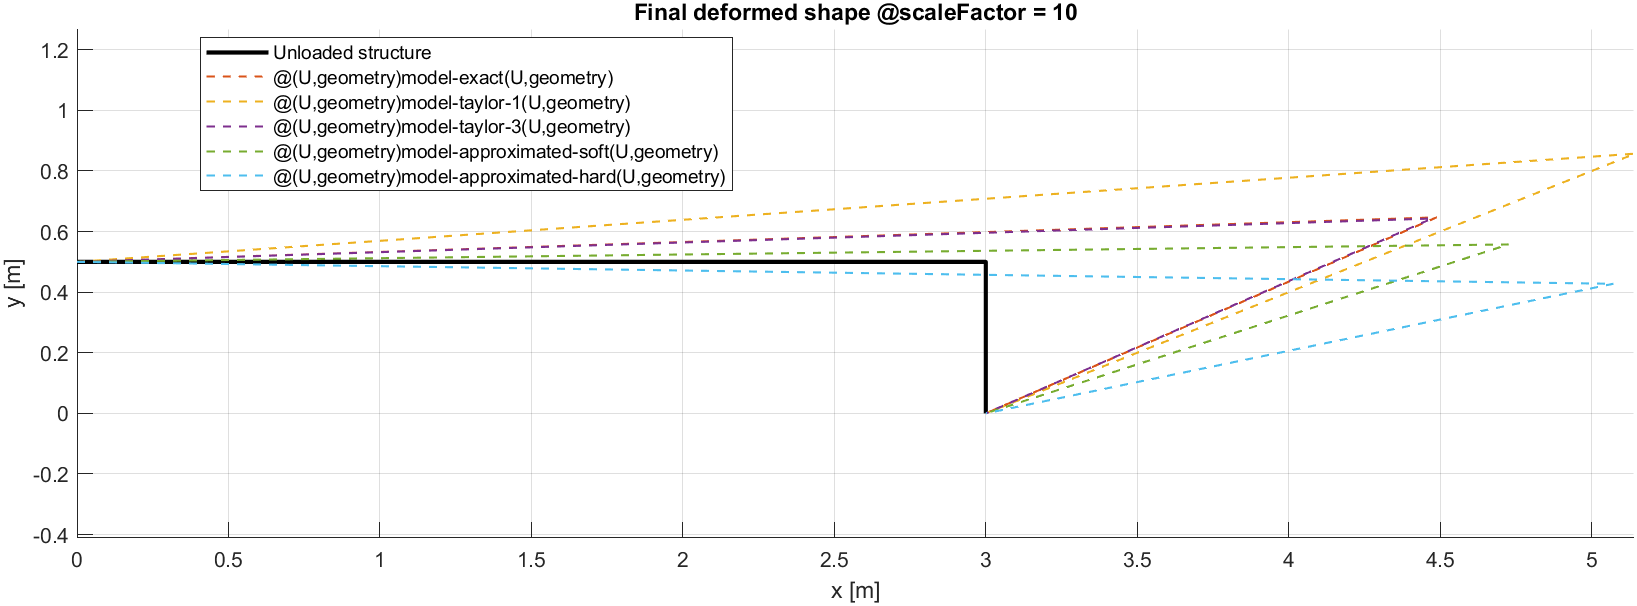
\includegraphics[width=.9\textwidth]{img/final_displacement_comparison_Px5000000_Py5000000}
    \caption{Comparison of final displacement for different models used}
    \label{fig:final_displacement_comparison}
\end{figure}

\begin{table}[H]
    \centering
    \begin{tabular}{|l|l|l|l|l|}
        \hline
        \textbf{Model name}     & \textbf{Px} & \textbf{Py} & \textbf{Ux} & \textbf{Uy} \\ \hline
        model-exact             & 5000000     & 5000000     & 1.49e-01    & 1.47e-02    \\ \hline
        model-taylor-1          & 5000000     & 5000000     & 2.14e-01    & 3.57e-02    \\ \hline
        model-taylor-3          & 5000000     & 5000000     & 1.47e-01    & 1.43e-02    \\ \hline
        model-approximated-soft & 5000000     & 5000000     & 1.73e-01    & 5.75e-03    \\ \hline
        model-approximated-hard & 5000000     & 5000000     & 2.07e-01    & -7.24e-03   \\ \hline
    \end{tabular}
    \caption{Numerical results for the different models used.}
    \label{tab:results_Px5000000_Py5000000}
\end{table}

As we can see, from the graph in Figure \ref{fig:final_displacement_comparison} and from the table in Table \ref{tab:results_Px5000000_Py5000000}, the final displacement for the different models used varies a lot.
This behavior is due to the fact that the different models were obtained under the assumption of small displacements.
When the displacements becomes bigger (due to high loads), the different models started to diverge from the exact one.

It's also interesting to understand how the different models behave differently for a set of different loads.
This means to analyze the trajectory of point $B$ predicted by the different models.

\begin{figure}[H]
    \centering
    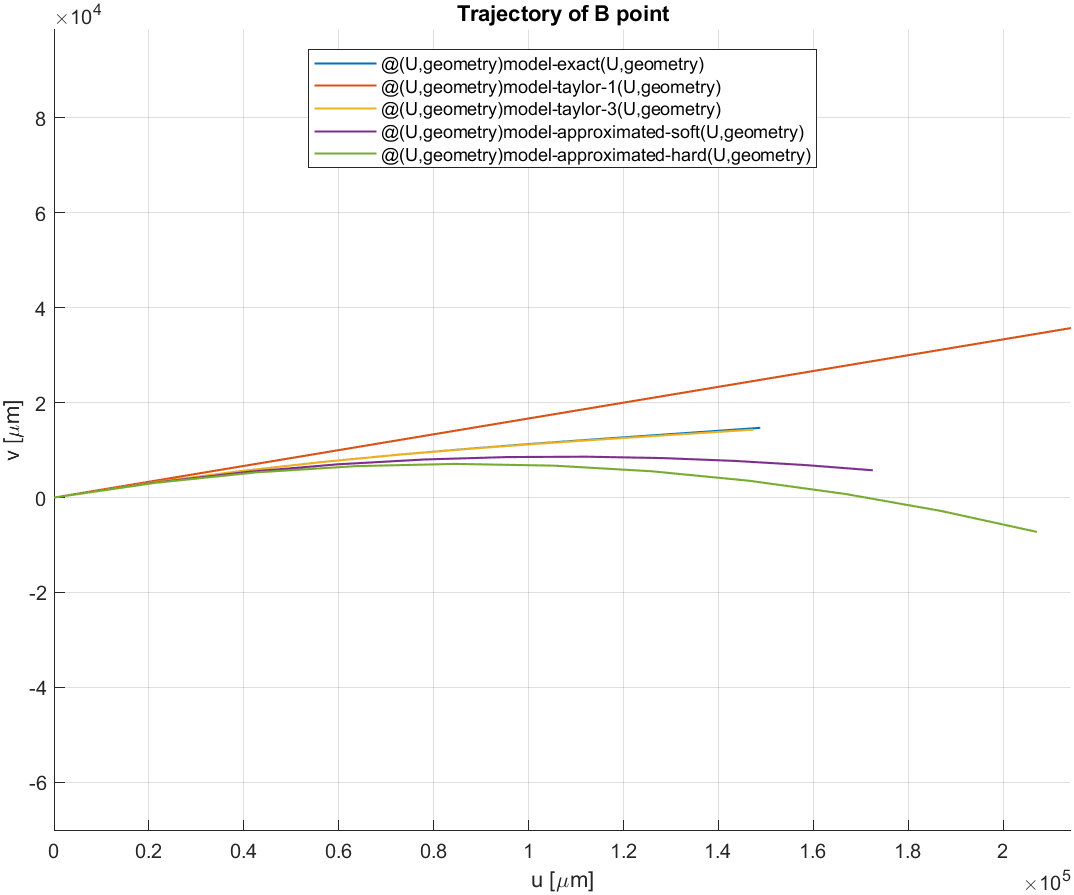
\includegraphics[width=.7\textwidth]{img/trajectory_comparison_Px5000000_Py5000000}
    \caption{Comparison of trajectory for the different models used}
    \label{fig:trajectory_comparison}
\end{figure}

From the graph in Figure \ref{fig:trajectory_comparison} we can appreciate the behavior of the linearized models based on the Taylor's order used.

Also, we can appreciate how the approximated models start to diverge and assume a completely wrong trajectory that is of course not feasible in the real world.

\begin{figure}[H]
    \centering
    \begin{subfigure}[b]{0.45\textwidth}
        \centering
        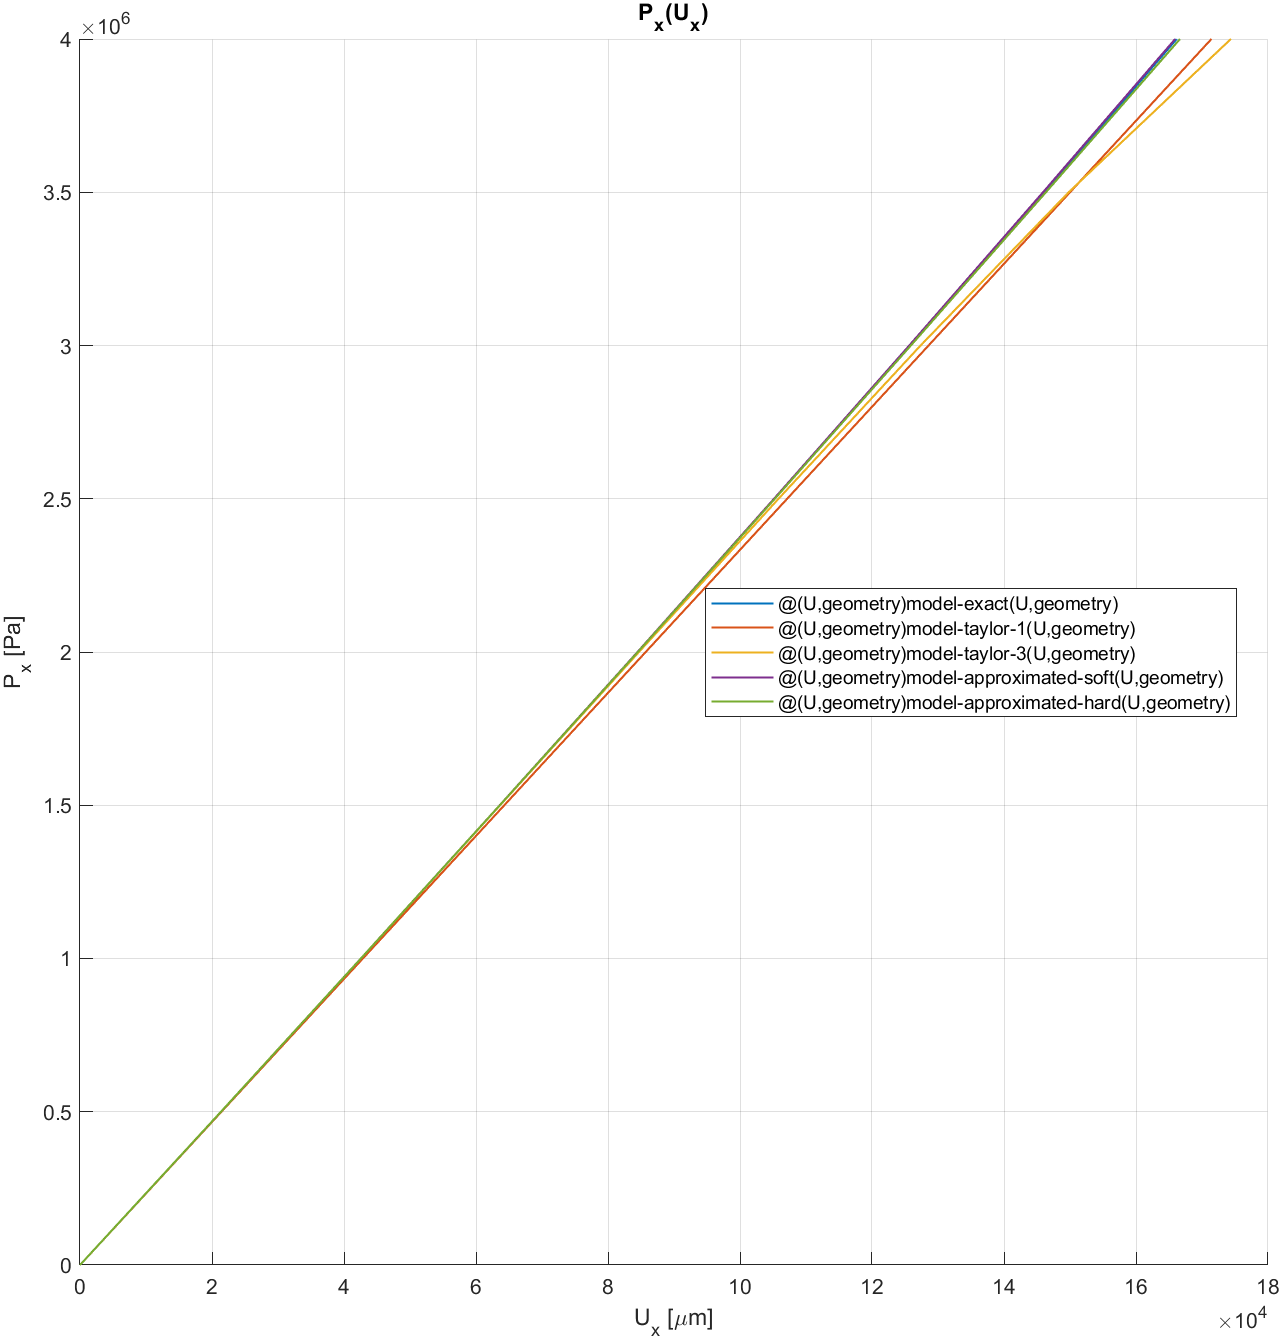
\includegraphics[width=.9\textwidth]{img/force_versus_displacement_Px5000000_Py0}
        \caption{Force versus displacement $P_x(u_x) @ P_y = 0$}
        \label{fig:force_versus_displacement_Px5000000_Py0}
    \end{subfigure}
    \hfill
    \begin{subfigure}[b]{0.45\textwidth}
        \centering
        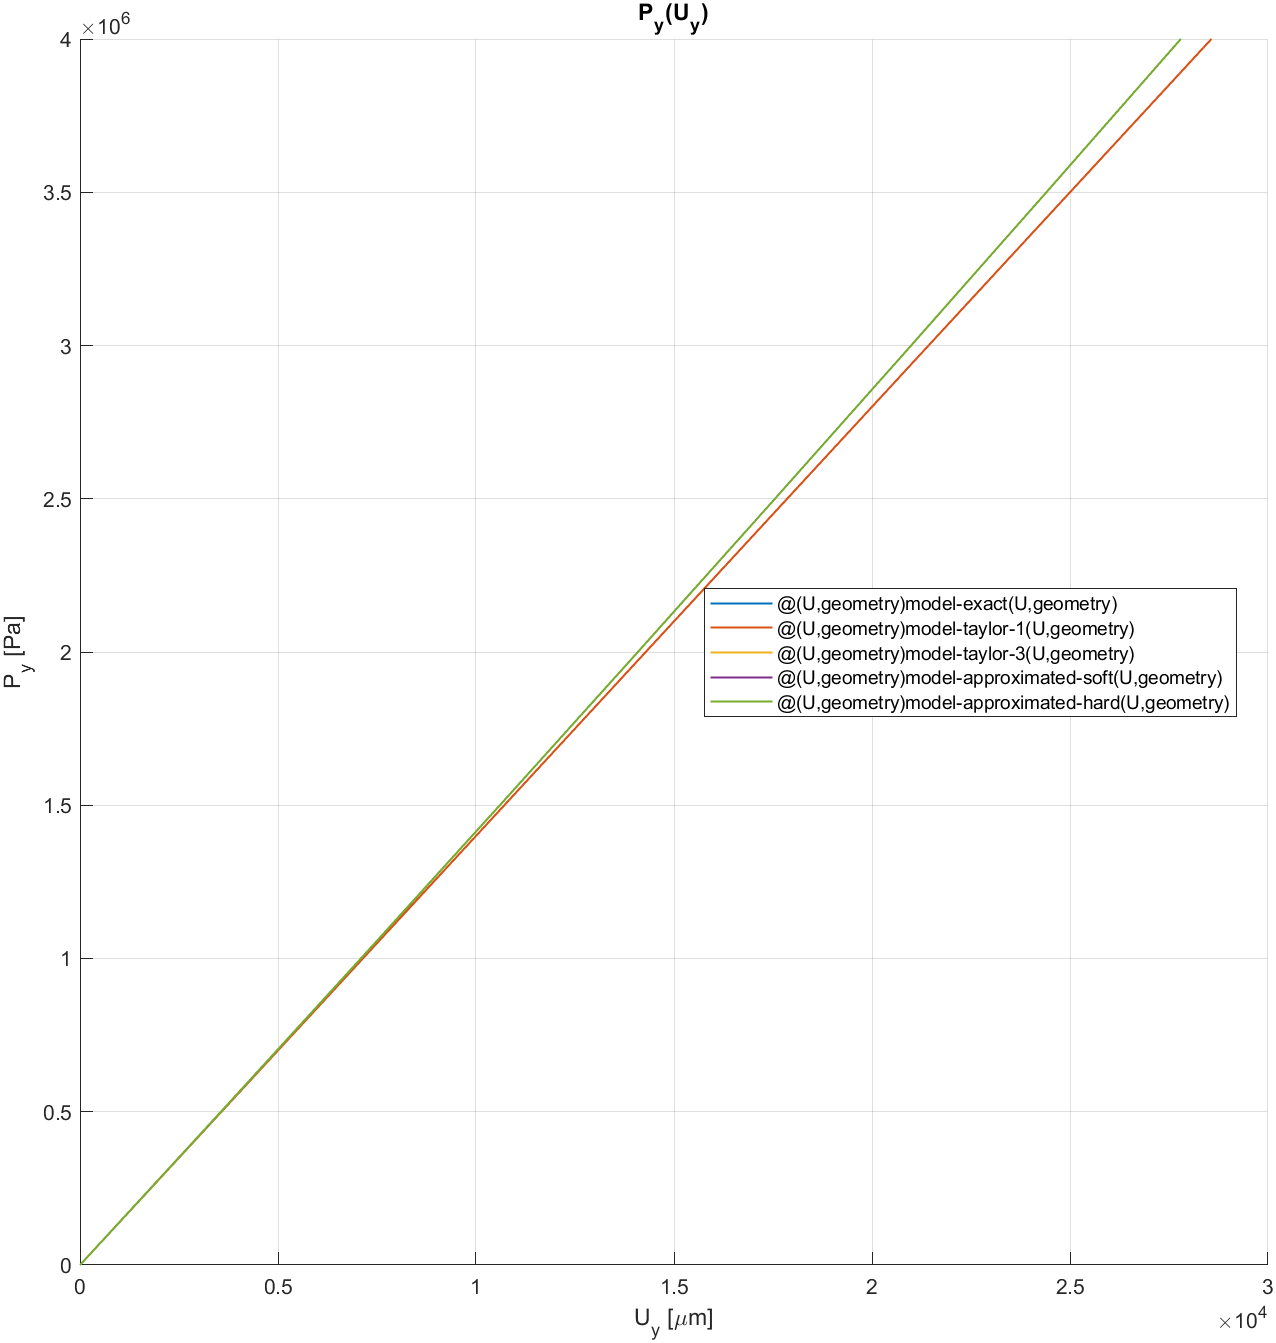
\includegraphics[width=.9\textwidth]{img/force_versus_displacement_Px0_Py5000000}
        \caption{Force versus displacement $P_y(u_y) @ P_x = 0$}
        \label{fig:force_versus_displacement_Px0_Py5000000}
    \end{subfigure}
\end{figure}

As we can see from the graph in Figure \ref{fig:force_versus_displacement_Px5000000} and in Figure \ref{fig:force_versus_displacement_Py5000000}, the error / divergence between the different models increases with the load (as expected).

\begin{figure}[H]
    \centering
    \begin{subfigure}[b]{0.45\textwidth}
        \centering
        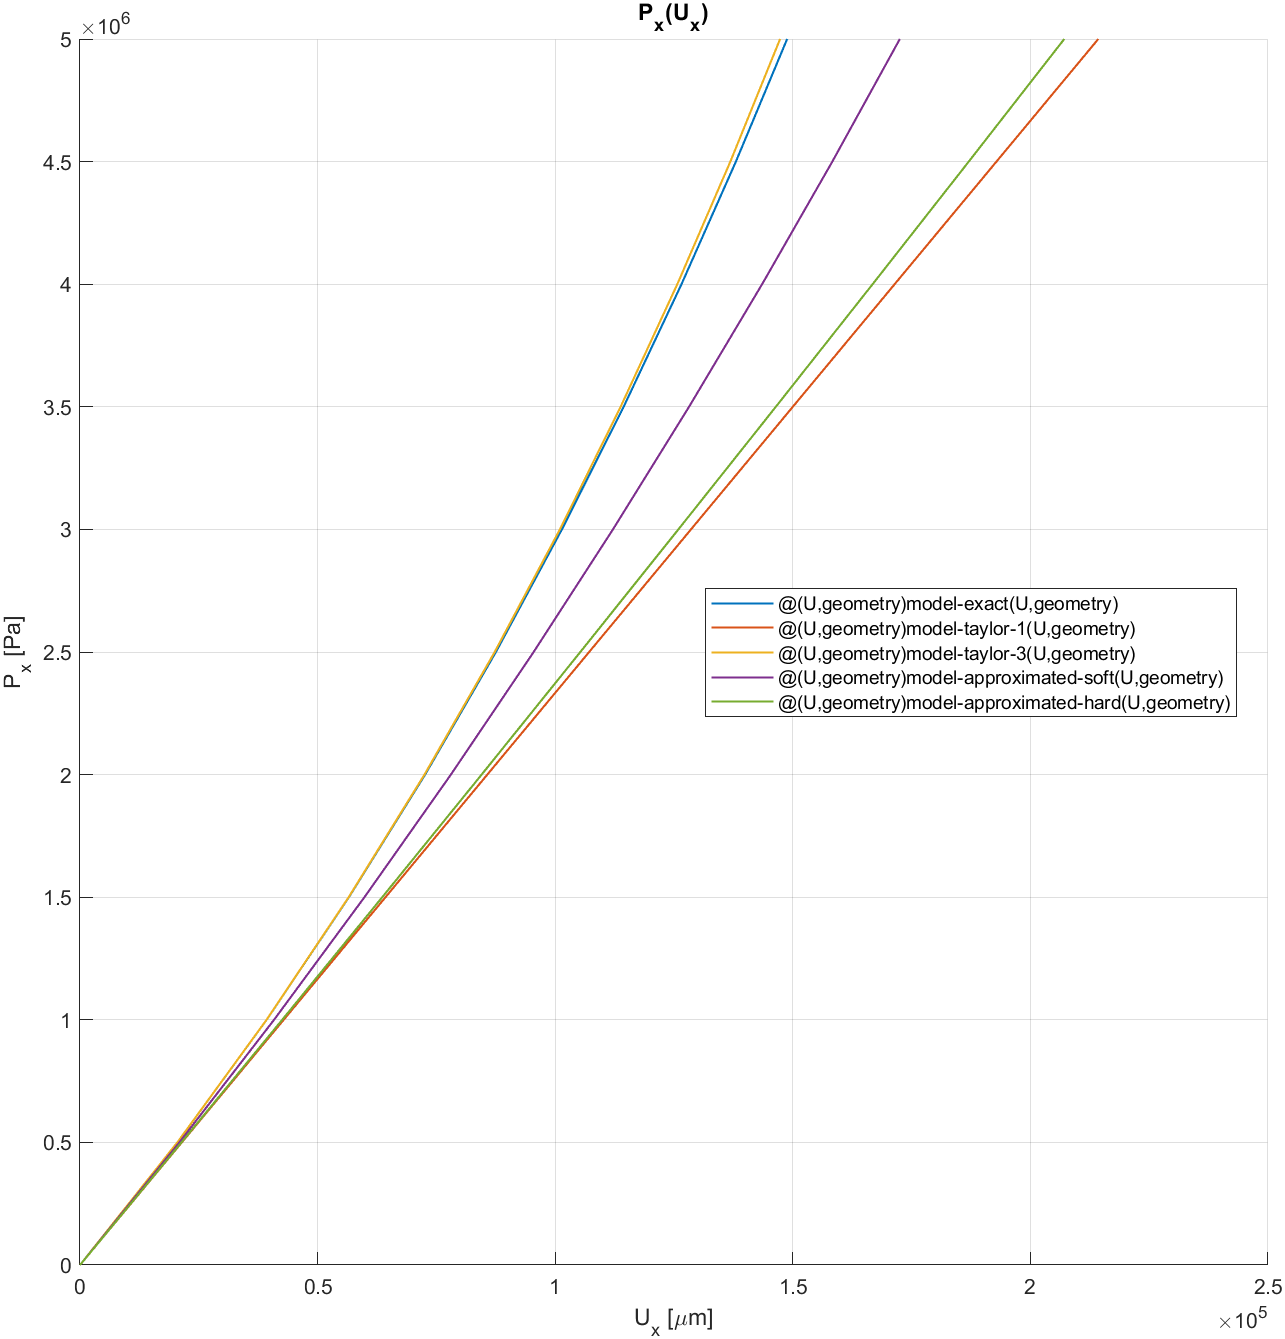
\includegraphics[width=.9\textwidth]{img/force_versus_displacement_Px5000000}
        \caption{Force versus displacement $P_x(u_x)$}
        \label{fig:force_versus_displacement_Px5000000}
    \end{subfigure}
    \hfill
    \begin{subfigure}[b]{0.45\textwidth}
        \centering
        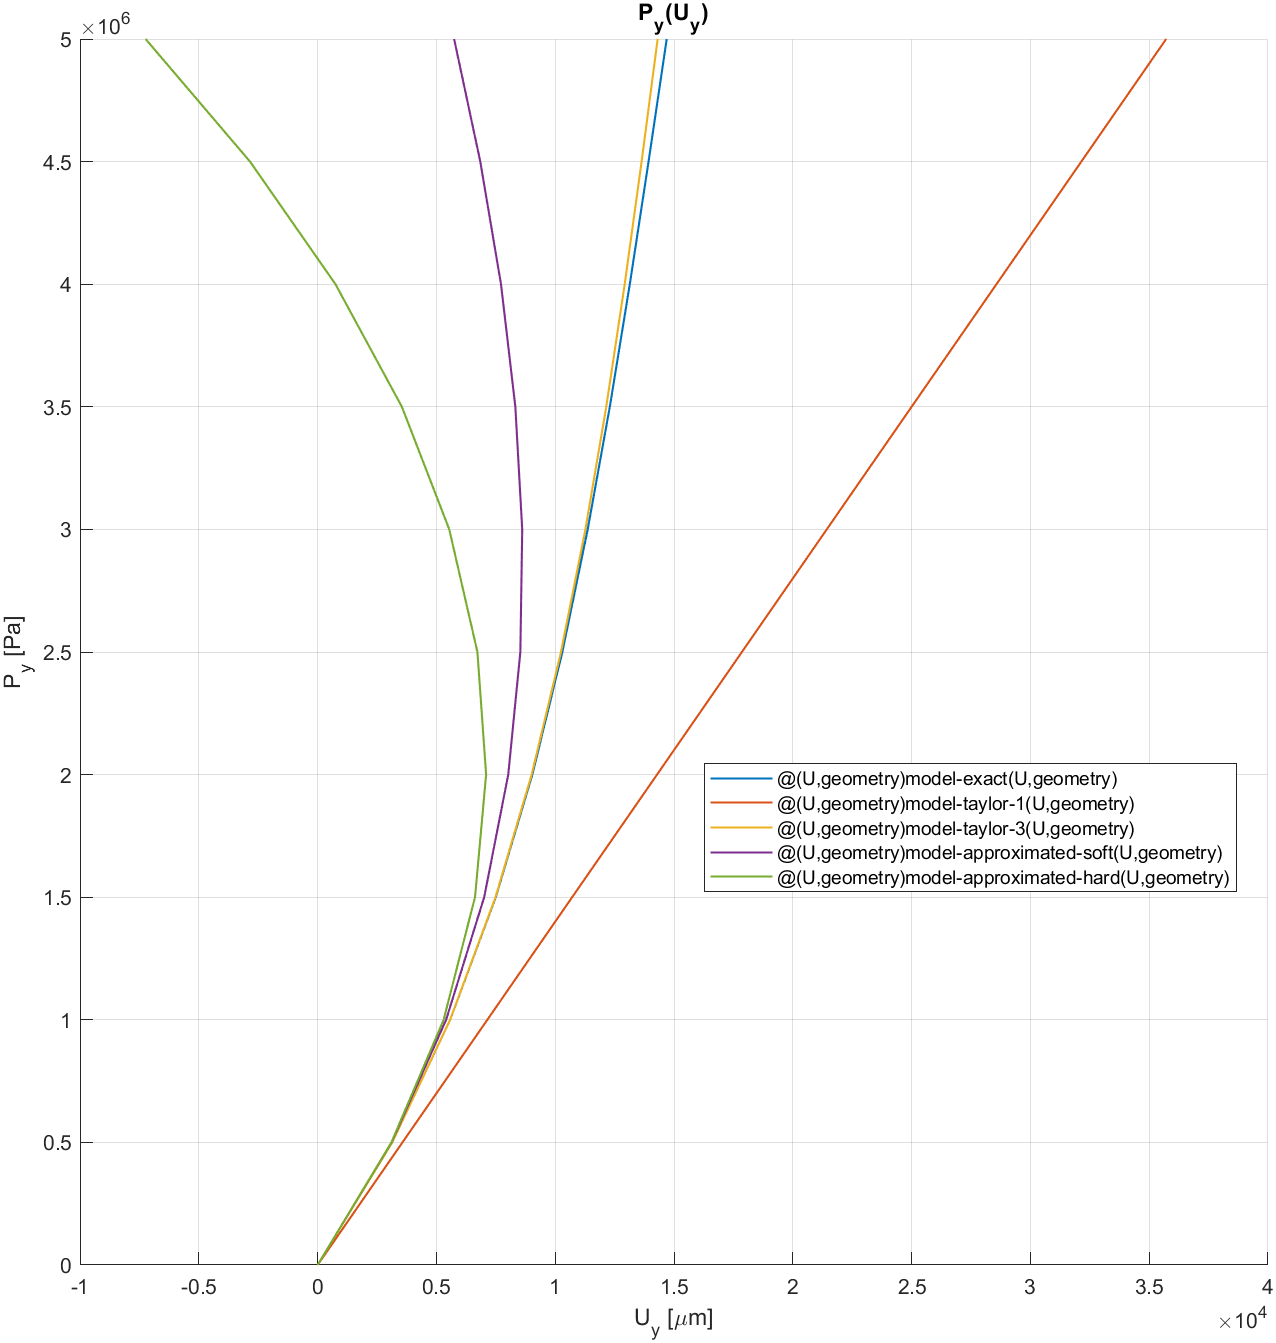
\includegraphics[width=.9\textwidth]{img/force_versus_displacement_Py5000000}
        \caption{Force versus displacement $P_y(u_y)$}
        \label{fig:force_versus_displacement_Py5000000}
    \end{subfigure}
\end{figure}

An interesting behavior of the model is observed under very high loads.
In fact, if we plot the same graph as in Figure \ref{fig:force_versus_displacement_Px5000000_Py0} and in Figure \ref{fig:force_versus_displacement_Px0_Py5000000} but without keeping zeroing the other load, we can see that the model starts to behave differently.
In particular, all the curves force versus displacement get more inclined and eventually start to have a negative slope.
This trend is clearly visible for the approximated models.

Another way to visualize this behavior is in Figure \ref{fig:trajectory_comparison} and in Figure \ref{fig:final_displacement_comparison}, where in both cases we can clearly see the approximated models diverging to a negative $v$ displacement.
Remember that the applied loads $P_x$ and $P_y$ are both positive, so the negative displacement is not a feasible solution.
What causes this behavior is still unknown and will probably be investigated in the future.